\chapter{Ricevitori multi protocollo}
\label{capitolo4}
\thispagestyle{empty}
In questo capitolo tratteremo la progettazione e la realizzazione del nuovo  ricevitore per la ricezione degli allarmi tramite vettori TCP/IP sfruttando sia le normali linee ADSL sia quelle GPRS.
\section{Nuovi vettori di comunicazione: dal PSTN al TCP/IP}
Con la diffusione della fibra ottica e delle comunicazione VoIP sono sempre meno le tradizionali linee PSTN che permettono la comunicazione di messaggi tramite i toni. Si è deciso perciò di passare alla comunicazione TCP/IP per comunicare gli eventi di allarme. Questo tipo di comunicazione permette di utilizzare sia connessioni ADSL che connessioni GPRS senza dover modificare nulla per quanto riguarda i protocolli di trasmissione.\\
Per poter utilizzare questa tipo di vettori di comunicazione sono stati adattati tre protocolli,uno standard e due proprietari per la trasmissione dei dati su TCP/IP. Il primo permette la ricezione direttamente dalle centrali di allarme, gli altri due permettono la comunicazione con i ricevitori proprietari corrispondenti. Questi protocolli sono:
\begin{itemize}
	\item SIA over IP
	\item Urmet AteArgo
	\item Bentel Visonic
\end{itemize}
\subsection{SIA over IP}
Per l'analisi e lo studio del protocollo si è fatto riferimento a due documenti della Security Industry Assocation, questi documenti sono ANSI/SIA DC-09-2007\cite{dc09} per la trasmissione di eventi sulla rete internet e ANSI/SIA DC-07-2001\cite{dc07} che descrive l'interfaccia di comunicazione.
Questo protocollo permette la comunicazione delle informazioni su linee ADSL o GPRS utilizzando lo stesso pacchetto tuttavia la rappresentazione dell'informazione si basa su due vecchi protocolli utilizzati per PSTN; questi due protocolli sono il SIA e il Contact ID. Partiremo perciò con la nostra trattazione con la struttura del pacchetto che è uguale in entrambi i casi.
\subsubsection{La struttura del pacchetto}
Il pacchetto di trasmissione è così formato:
$$
\begin{array}{c}
\langle LF\rangle\langle CRC\rangle\langle 0LLL\rangle\langle ''ID''\rangle\langle Sequence\#\textbf{!}segment\#|\rangle\\\langle\textbf{R}reciver\rangle\langle\textbf{L}line\#\rangle
{[data]}\langle timestamp\rangle \langle CR\rangle\\
\end{array}	 
$$
Dove i campi indicati sono rispettivamente:
\begin{description}
	\item[LF:] indica il carattere esadecimale \texttt{0x0A} e sta ad indicare l'inizio del pacchetto;
	\item[CRC:] campo utilizzato per il controllo degli errori tramite un meccanismo di Cyclic Redundancy Check a 16 bit;
	\item[0LLL:] campo utilizzato per indicare la lunghezza del pacchetto. Essa è calcolata considerando come primo carattere le virgolette del campo ID e come ultimo il carattere '$ ] $';
	\item[''ID'':] il campo ID è una stringa che identifica la tipologia di messaggio contenuta nel campo \texttt{data} quelli più importanti per noi sono i tag:
	\begin{itemize}
		\item SIA-DCS,
		\item ADM-CID.
	\end{itemize}
	utilizzati per indicare che il messaggio contenuto nel campo \texttt{data} è un messaggio di allarme con la normale codifica SIA oppure Contact-ID;
	\item[Sequence\#\textbf{!}segment\#:] questo campo è composto da due sotto-campi il primo, \emph{Sequence} è un numero di quattro cifre obbligatorio e serve ad indicare il numero sequenziale del messaggio inviato, se questo valore è seguito dal carattere ''\texttt{!}'' allora è presente un secondo numero utilizzato soprattutto nel caso in cui il messaggio contenuto nel campo \texttt{data} fosse troppo lungo da non poter essere inviato in un solo messaggio;
	\item[\textbf{R}receiver:] questo campo è valore composto da un numero variabile di cifre precedute dalla lettera \texttt{R} che identificano chi sta trasmettendo, in molti casi questo valore coincide con il codice della centrale;
	\item[\textbf{L}line\#:] campo variabile composto dalla lettera \texttt{L} seguita da 1 a 6 cifre ed indica la linea di ricezione;
	\item[{[...data...]}:] stringa che contiene le informazioni da trasmettere essa è composta da una parentesi quadrata seguita dal numero identificativo della centrale preceduto dal carattere ''\#'' e seguito dal carattere ''\texttt{|}'', dopo questo carattere è presente la vera informazione del messaggio, il delimitatore di fine stringa è una parentesi quadrata chiusa;
	\item[timestamp:] un campo non obbligatorio che indica l'istante in cui il messaggio è stato accodato per l'invio, esso ha la seguente formattazione autoesplicativa
	\begin{center}
		\texttt{\_HH:MM:SS,MM-DD-YYYY}
	\end{center}
	\item[CR:] è il delimitatore finale del pacchetto e corrisponde al carattere ASCII corrispondente al valore esadecimale \texttt{0x0D}			
\end{description}
Con lo standard DC09 viene introdotto anche un campo supplementare tra quello \texttt{data} ed il \texttt{timestamp} questo campo, denominato \texttt{xdata}, è compreso tra parentesi quadrata ed estende la potenza di espressione del protocollo. Il campo \texttt{xdata} inizia sempre con un carattere ASCII maiuscolo compreso nel range ''G'' e ''Z'' il cui significato è mostrato in \tablename~\ref{tab:xdata}
\begin{table}
	\begin{tabularx}{\linewidth}{|l|c|X|}
		\hline
		\textbf{Nome} & \textbf{Id} & \textbf{Descrizione} \\
		\hline
		Tempo di occorrenza & ''H'' & Timestamp nel quale si è verificato l'evento\\
		\hline
		MAC Address & ''M'' & Mac address del dispositivo trasmettitore\\
		\hline
		Verifica & ''V'' & Informazioni riguardo ad audio o video associate l'evento\\
		\hline
		Testo di allarme & ''I'' & Breve testo che contiene informazioni riguardanti l'allarme o un commento\\
		\hline
		Nome del sito & ''S'' & Nome del sito nel quale è avvenuto l'allarme\\
		\hline
		Nome dell'edificio & ''O'' & Etichetta che contiene informazioni riguardanti l'edificio che ha generato l'evento.\\
		\hline
		Luogo & ''L'' & Indicazione precisa di dove è avvenuto l'evento segnalato\\
		\hline
		Longitudine & ''X'' & Longitudine del luogo\\
		\hline
		Latitudine & ''Y'' & Latitudine del luogo\\
		\hline
		Altitudine & ''Z'' & Altitudine del luogo\\
		\hline
	\end{tabularx}
	\caption{Possibili valori iniziali per il campo \texttt{xdata}}\label{tab:xdata}
\end{table}
\subsubsection{La criptazione del pacchetto}
La struttura del pacchetto appena mostrata è utilizzabile così com'è in caso di comunicazione tra una centrale di allarme e un ricevitore in ambiente locale. Tuttavia quando le informazioni devono viaggiare attraverso internet è necessario che le informazioni siano protette in qualche modo. Per fare ciò lo standard DC09 prevede che i pacchetti siano criptati tramite algoritmo di criptazione AES che può utilizzare chiavi a 128, 192 o 256 bits.\\
Tuttavia non viene criptato l'intero pacchetto ma solamente il campo \texttt{data} dello stesso. Per indicare che il pacchetto è criptato si aggiunge il carattere ''*'' prima dell'etichetta nel campo ID.\\
Visto che la criptazione AES richiede che il pacchetto da criptare sia di lunghezza multipla di 16 per rispettare questo vincolo lo standard prevede l'inserimento di un campo \texttt{pad} composto da caratteri random tra il carattere ''['' e il campo account all'interno del campo \texttt{data}.\\
Secondo lo standard è necessario che il software di ricezione implementi la criptazione tramite una qualsiasi delle tre chiavi, tuttavia nel nostro caso abbiamo implementato solo la criptazione con chiave a 128 bit lasciando ad una futura implementazione le altre due chiavi. Questa supposizione è valida in quanto le centrali di un determinato fabbricante implementano solamente un tipo di criptazione.
\subsubsection{La connessione}
Lo standard DC09 prevede che la connessione tra il ricevitore e la centrale possa avvenire sia tramite l'utilizzo dello \emph{User Data Protocol} (UDP) sia tramite l'utilizzo del \emph{Transmission Control Protol} (TCP), il ricevitore da noi implementato permette attualmente solo l'utilizzo della modalità TCP, in quanto la modalità UDP è meno diffusa ed implementata tramite hardware con una scheda di espansione per il ricevitore System III.\\
Da notare il fatto che per la trasmissione tramite UDP nell'header del messaggio è necessario introdurre la porta della centrale d'allarme sulla quale il ricevitore dovrà inviare la risposta al messaggio.
In \fname{fig:transmission} vediamo la sequenza di messaggi che avviene durante la trasmissione di un evento.
\begin{figure}
	\centering
	\subfigure[]
	{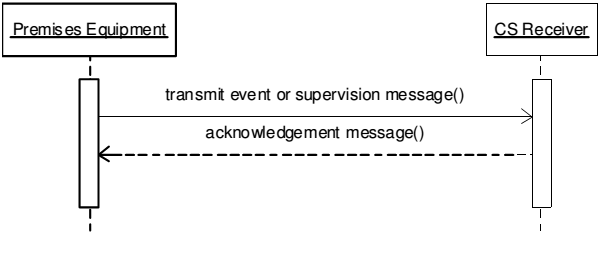
\includegraphics[width=7cm]{pictures/udp.png}\label{fig:udp}}
	\hspace{5mm}
	\subfigure[]
	{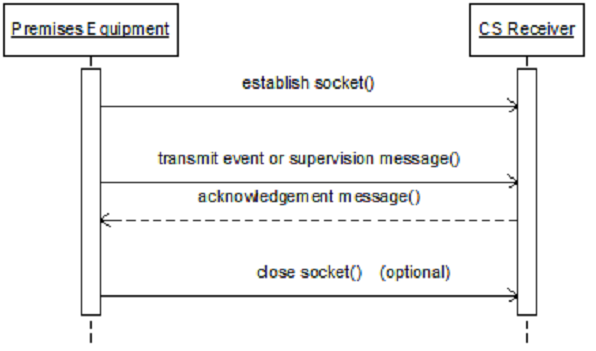
\includegraphics[width=6.5cm]{pictures/tcp.png}\label{fig:tcp}}
	\caption{Esempio di trasmissione UDP \ref{fig:udp} e TCP \ref{fig:tcp} }\label{fig:transmission}
\end{figure}
\subsubsection{I tipi di pacchetto}
Dopo aver visto come sono strutturati i pacchetti di informazione vediamo ora quali informazioni possono essere trasmesse da questi pacchetti.
Lo standard prevede una classificazione per le tipologie di pacchetti, in particolare si distinguono tre classi principali:
\begin{itemize}
	\item Event Messages
	\item Supervisor Messages
	\item Acknowledgement Messages
\end{itemize}
Inoltre lo standard DC07 prevede per uno sviluppo futuro dei messaggi di \emph{data/operation request} pensati per essere inviati dal ricevitore per richiede lo svolgimento di alcune operazioni o lo stato di alcuni componenti.
\paragraph{Event messages}
Gli event messages sono quei messaggi inviati dalla centrale di sicurezza per comunicare degli eventi al ricevitore. Essi rispettano lo standard appena descritto, il campo \texttt{ID} di questo tipo di messaggi può essere uno dei seguenti:
\begin{itemize}
	\item SIA-DCS
	\item ADM-CID
	\item SIA-PUL
	\item ACR-SF
	\item ADM-41E
	\item FBI-SF
	\item SK-FSK1
\end{itemize}
tuttavia gli unici tag che noi supporteremo saranno quelli del SIA-DCS e ADM-CID i quali sono anche gli unici obbligatori secondo lo standard.
\paragraph{Supervisor message}
Questo tipo di messaggi non sono obbligatori, tuttavia sono molto consigliati, in quanto permettono di monitorare periodicamente lo stato della connessione. Questi messaggi sono inviati periodicamente dalla centrale di allarme al ricevitore, il tempo tra una trasmissione e l'altra può essere impostato secondo lo standard da un minimo di 10 secondi ad un massimo di 1080 ore. Se nessun tipo di messaggio raggiunge il ricevitore in questo intervallo di tempo la comunicazione fallisce e il ricevitore dovrebbe segnalare la mancata comunicazione, inoltre, un evento di mancata comunicazione dovrebbe essere registrato dalla centrale.\\
Quando il sistema di supervisione è attivo, periodicamente la centrale invia un messaggio strutturato come in precedenza ma con \texttt{ID} uguale a \emph{NULL} e campo \texttt{data} vuoto. Un esempio di messaggio è il seguente:
$$
\begin{array}{c}
\langle LF\rangle\langle CRC\rangle\langle 0LLL\rangle\langle ''NULL''\rangle\langle 0000\rangle\\\langle\textbf{R}recv\rangle\langle\textbf{L}pref\rangle
{[]}\langle timestamp\rangle \langle CR\rangle\\
\end{array}	 
$$
\paragraph{Acknowledgment message}
Quando il ricevitore riceve dalla centrale un evento esso deve rispondere con un messaggio che può essere di quattro tipi:
\begin{itemize}
	\item ACK
	\item NAK
	\item DUH
	\item RSP
\end{itemize}
Il messaggio di ACK corrisponde ad una risposta positiva e viene inviato quando il ricevitore riceve correttamente l'evento senza errori, un esempio di messaggio di ACK è il seguente:
$$
\begin{array}{c}
\langle LF\rangle\langle CRC\rangle\langle 0LLL\rangle\langle ''ACK''\rangle\langle seq\rangle\\\langle\textbf{R}recv\rangle\langle\textbf{L}pref\rangle
{[]}\langle timestamp\rangle \langle CR\rangle\\
\end{array}	 
$$
dove i campi \texttt{seq}, \texttt{recv} e \texttt{pref} vengono copiati dal messaggio originale al quale si vuole dare una risposta.\\
Il messaggio di NAK è simile a quello di ACK tuttavia cambia il campo \texttt{ID} e il numero di \texttt{seq} che viene impostato a 0000, un esempio è riportato di seguito.
$$
\begin{array}{c}
\langle LF\rangle\langle CRC\rangle\langle 0LLL\rangle\langle ''NAK''\rangle\langle 0000\rangle\\\langle\textbf{R}recv\rangle\langle\textbf{L}pref\rangle
{[]}\langle timestamp\rangle \langle CR\rangle\\
\end{array}	 
$$
Il pacchetto DUH viene inviato nel caso in cui il ricevitore, pur avendo verificato che il pacchetto è formattato correttamente e non contiene errori, non è in grado di tradurlo o comunque di interpretare la richiesta. In questo caso i campi \texttt{seq}, \texttt{recv} e \texttt{pref} sono uguali a quelli della richiesta ricevuta.\\
Il pacchetto RSP è stato introdotto come pacchetto di risposta per i messaggi di data/operation request tuttavia come questi pacchetti è pensato per un uso futuro. A differenza dei pacchetti precedenti il campo \texttt{data} contiene dei valori. Il numero di sequenza, del ricevitore e della linea sono copiati dal pacchetto di richiesta.
\subsection{Urmet AteArgo}
Il protocollo in questione è un protocollo proprietario di Urmet che serve per connettere il nostro sistema ad un ricevitore che permetta la gestione delle periferiche Webu All-In-One viste nel \chaptername \ref{capitolo2}. Questa integrazione si è resa necessaria per cercare di dismettere il software proprietario di Cobra, lo \emph{MTSfe}.\\
Essendo il protocollo proprietario non potremmo addentrarci in modo approfondito nel protocollo come nel precedente caso, tuttavia analizzeremo il funzionamento e la struttura generale del pacchetto.
\subsubsection{La struttura del pacchetto}
A differenza del protocollo precedente questo è un protocollo XML, ovvero, i pacchetti non sono alto che un unica stringa di caratteri che forma una strutta XML.
Il pacchetto è formato da un tag iniziale che delimita l'inizio del pacchetto, seguito da un \texttt{header} nel quale sono contenuti data e ora dell'evento. La parte di header è seguita dalla vera e propria informazione della segnalazione, questa parte denominata \texttt{body} ha un attributo che ne identifica il tipo di pacchetto trasmesso. All'interno del campo body, nel caso si tratti di una notifica di evento abbiamo tutte le informazioni riguardo la centrale che ha generato l'evento come il codice identificativo o i tipi di allarme generati. A differenza del protocollo precedente, è possibile inviare più eventi nello stesso pacchetto riguardanti anche zone diverse della stessa centrale. Inoltre, visto che la Webu All-In-One fornisce anche la funzione di ''ponte PSTN'' è possibile che vengano inviati eventi riguardanti sia la centrale di allarme principale che eventi generati dalla Webu in un unico pacchetto.\\
A differenza del protocollo precedente e di quello che analizzeremo in seguito in questo capitolo quello di AteArgo non prevede l'utilizzo di codici Contact ID o SIA è stato quindi necessario prevedere anche un meccanismo di traduzione.
\subsubsection{La connessione}
La connessione diretta con le periferiche Webu è gestita dal ricevitore software AteArgo perciò la nostra connessione è di tipo locale con quest'ultimo software. Dato che le informazioni viaggiano su una rete locale esse sono potenzialmente protetta tramite altri meccanismi perciò gli sviluppatori di Urmet non hanno incluso la criptazione del pacchetto.\\
La connessione con AteArgo è una connessione di tipo client-server dove il software AteArgo ricopre il ruolo di server e risponde a specifiche richieste è perciò necessario prevedere un meccanismo di \emph{polling} per la ricezioni degli eventi, infatti, gli eventi saranno comunicati solamente come risposta ad una richiesta da parte del nostro software. Nel caso in cui vi siano eventi il software risponde con un pacchetto di eventi altrimenti il sistema risponde con un pacchetto di ACK.
Nella \fname{fig:comateargo} è mostrato il meccanismo di comunicazione tra i due software.
\begin{figure}
	\centering
	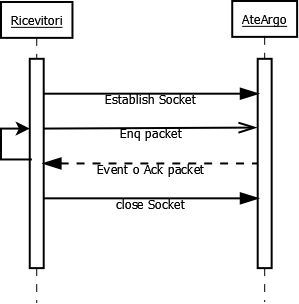
\includegraphics[width=0.5\linewidth]{pictures/conateargo.png}
	\caption{Comunicazione tra il software di ricezione e il software AteArgo}\label{fig:comateargo}
\end{figure}
\subsubsection{I tipi di pacchetto}
In questo caso non possiamo addentrarci in particolare sulle tipologie di pacchetto che possiamo trovare nel protocollo tuttavia possiamo fare alcune distinzioni, i pacchetti che sicuramente incontriamo sono quattro:
\begin{itemize}
	\item pacchetto di enquiry (richiesta);
	\item pacchetto di acknowledgment;
	\item pacchetto di evento;
	\item pacchetto di comando.
\end{itemize}
\paragraph{Pacchetto di enquiry}
Questo tipo di pacchetto è utilizzato dal client per richiedere informazioni al server. In questo caso il client ciclicamente continua ad inviare al server questo pacchetto ed il server può rispondere con un messaggio di acknowledgment o con un messaggio di evento.\\
Il blocco body di questo messaggio è praticamente vuoto se non per alcune informazioni riguardanti ora e data della richiesta necessarie per la sincronia con il server.
\paragraph{Pacchetto di acknowledgment}
In questo caso il pacchetto è inviato dal server al client ed è la risposta ad un messaggio di enquiry nel caso non vi siano eventi da segnalare oppure in risposta ad un messaggio di comando, per confermare la corretta presa in carico della richiesta del client da parte del server.\\
Il blocco body di questo messaggio è praticamente vuoto se non per alcune informazioni riguardanti ora e data della richiesta necessarie per la sincronia con il server.
\paragraph{Pacchetto di evento}
Questo pacchetto è la risposta del server ad un messaggio di enquiry del client. In questo caso il messaggio contiene informazioni riguardo la centrale che ha generato un evento, su quale ingresso ha generato lo specifico evento ed un codice numerico che identifica la tipologia di evento generato. Inoltre, nel pacchetto vengono trasportate le informazioni che permettono di identificare se l'evento è stato generato dalla periferica Webu oppure, se è stato generato direttamente dalla centrale ed è passato tramite il ponte PSTN.
\paragraph{Pacchetto di comando}
Questa tipologia di pacchetto è inviata dal client verso il server per richiedere di eseguire un operazione su di una specifica periferica. Le operazioni che possono essere eseguite sono diverse tra cui l'impostazione della data e dell'ora sulla periferica, oppure l'attivazione o la disattivazione di un uscita o ancora l'esclusione di un ingresso.\\
In dettaglio ritorneremo su questo pacchetto nel capitolo successivo nel quale tratteremo la telegestione.
\subsection{Bentel Visonic}
In questo caso parliamo  di un protocollo utilizzato per ricevere segnalazioni dalle centrali della serie \emph{BW} tramite l'ausilio del ricevitore Visonic sempre fornito da Bentel. La particolarità di questa serie di centrali è la possibilità di associare ad un evento alcune immagini provenienti direttamente dai sensori IR e non da un impianto di videosorveglianza.
\subsubsection{La struttura del pacchetto}
Anche in questo caso il pacchetto non è altro che una stringa composta da tag XML. Tuttavia questa volta i pacchetti che possiamo ricevere sono solamente pacchetti di eventi, di immagini o di controllo delle connessione ai quali rispondiamo con pacchetti di acknowledgment.\\
La struttura del pacchetto è molto semplice, dopo un tag di apertura del pacchetto vi è una parte che identifica l'evento e la centrale che lo ha trasmesso, dopo queste informazioni in base al tipo di pacchetto possiamo avere diversi tag che rappresentano i diversi tipi di pacchetto, essi possono essere tag di \texttt{heartbeat}, di \texttt{frame} o di \texttt{event}.
\subsubsection{La connessione}
La connessione tra il nostro software e il ricevitore Visonic avviene tramite una connessione TCP/IP di tipo client-server, in questo caso il nostro software ha il ruolo di server ed è il ricevitore Visonic che effettua la connessione.\\
Per monitorare la connessione il ricevitore invia periodicamente dei pacchetti, in caso questi pacchetti non arrivino per un determinato intervallo di tempo si può identificare un problema nella connessione o direttamente nel ricevitore. Questi pacchetti che analizzeremo nel paragrafo successivo sono detti di \emph{HeartBeat}. Un esempio del funzionamento è mostrato in \fname{fig:convisonic}
\begin{figure}
	\centering
	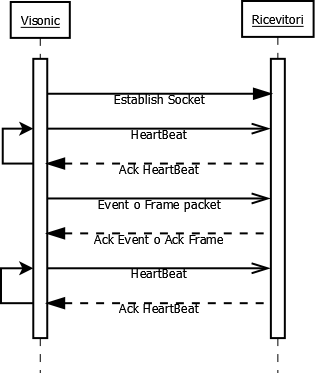
\includegraphics[width=0.5\linewidth]{pictures/convisonic.png}
	\caption{Comunicazione tra il software di ricezione e il software Visonic}\label{fig:convisonic}
\end{figure}
\subsubsection{I tipi di pacchetto}
I pacchetti che il ricevitore Visonic scambia con il nostro ricevitore sono di tre tipi:
\begin{itemize}
	\item pacchetto di HeartBeat;
	\item pacchetto di evento;
	\item pacchetto di frame.
\end{itemize}
Il nostro ricevitore risponde a questi messaggi con una risposta di ACK. Analizziamo ora, per quanto possibile i diversi pacchetti.
\paragraph{Pacchetto di HeartBeat}
Questo pacchetto serve a monitorare la connessione e in caso di problemi a ristabilirla. Esso ha la stessa struttura XML di un pacchetto d'evento tuttavia il suo contenuto è vuoto. In esso compaiono solo i tag che lo identificano come un pacchetto di heartbeat. Questo tipo di pacchetto viene inviato periodicamente al nostro software ricevitore. Nel caso in cui questo pacchetto non arrivi per un determinato periodo di tempo si può supporre che vi siano problemi con la connessione o più probabilmente con il ricevitore, si potrebbero prevedere perciò delle contromisure da mettere in atto quando questa situazione si verifica.
\paragraph{Pacchetto di evento}
Questo tipo di pacchetto viene inviato dal ricevitore Visonic quando un evento viene comunicato da una centrale, ogni pacchetto inviato contiene un unico evento che viene codificato sia tramite il protocollo proprietario Visonic sia tramite una stringa formattata secondo il protocollo Contact-ID.
Per noi risulta più semplice tradurre la stringa formattata in questo formato in quanto il resto del sistema lavora sfruttando questi codici e avremmo comunque dovuto effettuare una traduzione di questo tipo.
\paragraph{Pacchetto di frame}
Questo particolare pacchetto è utilizzato per trasmettere le immagini provenienti dal sensore che ha generato l'allarme in particolare il pacchetto che viene generato è composto dalla prima parte nella quale viene riportato un identificativo dell'evento alla quale l'immagine è associata e all'interno dei tag \texttt{frame} viene codificata l'immagine proveniente dal sensore.\\
Per ogni evento si possono avere da uno a cinque fotogrammi, per ogni fotogramma generato viene inviato un pacchetto frame che conterrà anche il numero sequenziale del frame.
\paragraph{Pacchetto di acknowledgment}
Per ogni pacchetto appena visto il nostro ricevitore deve rispondere con un pacchetto di acknowledgment il quale sarà leggermente diverso per ogni tipologia di pacchetto ricevuto, infatti, l'acknowledgment per un pacchetto di heartbeat differisce dall'acknowledgment del pacchetto di event. In particolare i pacchetti di ACK sono strutturati come i corrispettivi pacchetti ricevuti con lo stesso id del pacchetto ricevuto ed il campo informativo vuoto.
\section{La struttura dati}
Come abbiamo detto nel \chaptername~\ref{capitolo3} uno dei nostri vincoli è quello di mantenere la retro compatibilità con il vecchio software di LIS fino al completo aggiornamento dei moduli. Per fare ciò è stato necessario mantenere la struttura dati precedente per far si che il resto del software potesse prelevare i dati senza nessuna complicazione. In particolare la tabella più importante per la ricezione degli eventi era quella \texttt{allarmi\_contact\_id} i cui campi si ricavano dallo script di creazione del \lname{lst:allarmicontactid}
\begin{lstlisting}[language=SQL,caption=Tabella allarmi\_contact\_id,label=lst:allarmicontactid]
CREATE TABLE allarmi_contact_id (
    ac_id integer NOT NULL DEFAULT nextval(('"allarmi_contact_id_seq"'::text)::regclass),
    ac_centrale character varying(20),
    ac_allarme character varying(10),
    ac_area bigint,
    ac_zona bigint,
    ac_giorno smallint,
    ac_mese smallint,
    ac_anno smallint,
    ac_ora smallint,
    ac_minuto smallint,
    ac_secondo smallint,
    ac_data_inserimento timestamp without time zone DEFAULT now(),
    ac_pending character(1) DEFAULT 's'::character varying,
    ac_porta_seriale integer,
    ac_n_ricevitore smallint,
    ac_n_gruppo smallint,
    CONSTRAINT allarmi_contact_id_pkey PRIMARY KEY (ac_id)
)
\end{lstlisting}
Come si nota i campi da compilare sono diversi anche se non tutti necessari. Il campo allarme contiene il codice Contact ID dell'allarme ricevuto, nel paragrafo successivo vedremo come questo meccanismo sia stato adattato per l'utilizzo anche dei codici di allarme SIA. Il campo \texttt{pending} serve al cp200\_3 per identificare quali allarmi sono già stati processati in quanto questa tabella mantiene anche lo storico giornaliero degli allarmi ricevuti.\\
Oltre a questa tabella si è deciso anche di aggiornare una serie di tabelle collegate tra loro che hanno la funzione di monitorare lo stato dei ricevitori. Nel vecchio software per verificare l'eventuale blocco di un thread, ogni qualvolta che una segnalazione giungeva ad uno dei ricevitori veniva aggiornato un campo nella tabella \texttt{seriale} il quale è collegato alla tabella \texttt{ricevitori}; questo collegamento è mostrato in \fname{fig:erricevitori}.
\begin{figure}
	\centering
	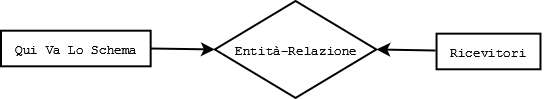
\includegraphics[width=0.8\linewidth]{pictures/erricevitori.png}
	\caption{Schema relazionale delle tabelle che controllano i ricevitori}\label{fig:erricevitori}
\end{figure}
Il codice di creazione di queste tabelle è mostrato nel \lname{lst:sqlricevitori}.

\begin{lstlisting}[language=SQL,caption=Tabelle ricevitori,label=lst:sqlricevitori]
CREATE TABLE seriale (
    se_id integer NOT NULL DEFAULT 	nextval(('"seriale_se_id_seq"'::text)::regclass),
    se_numero integer,
    se_stato character varying(1) DEFAULT 's'::character varying,
    se_allarme integer,
    se_controllo character varying(1),
    CONSTRAINT pk_seriale PRIMARY KEY (se_id)
)

CREATE TABLE ricevitore (
    ri_id integer NOT NULL DEFAULT nextval(('"ricevitore_ri_id_seq"'::text)::regclass),
    se_id integer,
    ri_stato character varying(2) DEFAULT 'n'::character varying,
    ri_tipo character varying(50),
    ri_batteria smallint,
    ri_modalita smallint,
    ri_mancanza_220 smallint,
    ri_stampante smallint,
    ri_collegato smallint,
    ri_data_220 timestamp with time zone,
    ri_data_batteria timestamp with time zone,
    ri_stato_ricevitore smallint,
    ri_numero smallint,
    CONSTRAINT pk_ricevitore PRIMARY KEY (ri_id),
    CONSTRAINT fk_ricevito_reference_seriale FOREIGN KEY (se_id)
    REFERENCES seriale (se_id) MATCH SIMPLE
    ON UPDATE RESTRICT ON DELETE RESTRICT
)
\end{lstlisting}
Il campo aggiornato da ogni ricevitore è il campo \texttt{se\_controllo} della tabella \texttt{seriale}.
Questa meccanismo se pur non necessario per il corretto funzionamento del vecchio software è stato mantenuto, con dei piccoli adattamenti, per monitorare il funzionamento del nuovo software di ricezione.
Tuttavia, come si nota dalla complessità delle tabelle, questo sistema porta con se anche degli elementi caratteristici del passato, come l'utilizzo di una tabella \texttt{seriale} utilizzata dai tempi in cui i ricevitori erano ancora collegati tramite questo tipo di connessione cablata.\\
In realtà la soluzione migliore sarebbe stata quella di rappresentare i ricevitori in un unica tabella, e per quelli che presentavano possibilità di multithreading aggiungere una tabella collegata a ricevitori che tenesse traccia dei thread aperti e nel caso di blocco di uno di questi mettesse in atto le opportune contromisure.

\section{Architettura e realizzazione del sistema}
Analizziamo ora come è stato sviluppato il sistema. Si è deciso di passare ad un software strutturato per classi. L'idea era quella di avere un controllore che monitorasse periodicamente i diversi ricevitori e nel caso questi non fossero avviati oppure bloccati li riattivasse in automatico. I ricevitori dal canto loro dovevano comportarsi tutti pressoché alla stessa maniera, ovvero, le funzioni principali da svolgere erano quella di:
\begin{itemize}
\item aggiornare il campo \texttt{controllo} della tabella \texttt{seriale};
\item caricare l'allarme sul database rispettando lo standard Contact ID e i diversi campi della tabella \texttt{allarmi\_contact\_id}
\end{itemize} 
inoltre al loro avvio dovevano creare ed aggiornare i diversi campi delle tabelle \texttt{seriale} e \texttt{ricevitore}. In \fname{fig:classiric} vediamo lo schema delle classi del software \texttt{Ricevitore}.
\begin{figure}[p]
	\centering
	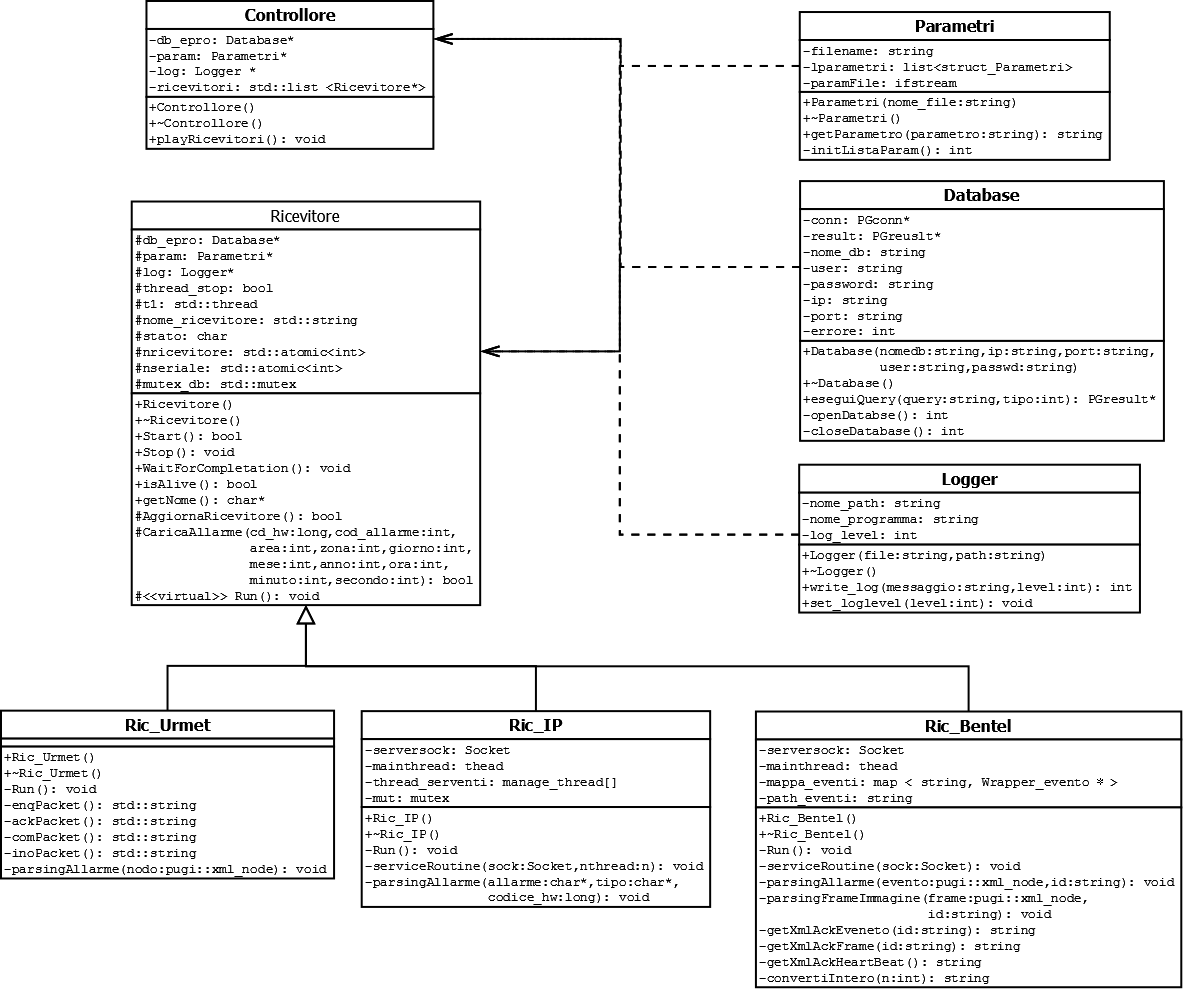
\includegraphics[height=\textwidth, angle=90]{pictures/classiric.png}
	\caption{Schema delle classi Ricevitori}\label{fig:classiric}
\end{figure}
\subsection{Le classi}
Analizziamo ora in dettaglio le classi principali del software di ricezione multi-ricevitore.
\subsubsection{Ricevitore}
La classe \texttt{Ricevitore} è una classe astratta che serve per generalizzare l'entità ricevitore, questa classe dovrà essere estesa ogni qualvolta si voglia integrare un nuovo ricevitore. Per quanto riguarda i suoi metodi i nomi sono abbastanza autoesplicativi, tuttavia in dettaglio il metodo \emph{AggiornaRicevitore} serve per controllare i valori nelle tabelle \texttt{Ricevitori} e \texttt{Seriale} in caso esistano già i valori corrispondenti non fa altro che aggiornare il campo \texttt{se\_controllo}, in caso contrario il metodo deve riempire la tabella con i valori assegnati dal ricevitore che invoca il metodo.\\
Il metodo \emph{CaricaAllarme}, invece, si occupa di caricare l'allarme proveniente da uno dei ricevitori sul database. Esso effettua semplicemente una query di \texttt{INSERT} nella tabella \texttt{allarmi\_contact\_id}. Per gestire la concorrenzialità delle interrogazioni al database è stato necessario prevedere un meccanismo di esclusione tramite l'utilizzo di un \emph{mutex} necessario per gestire l'esecuzione delle query in modo seriale. Inoltre sempre per impedire problemi di concorrenza gli attributi \texttt{nseriale} e \texttt{nricevitore} sono stati dichiarati \emph{atomici}.\\
Il metodo \texttt{Run} è il metodo astratto che deve essere implementato dalla classe figlia e contiene la routine che il thread deve eseguire e deve contenere tutta la logica di ricezione e parsing dell'allarme. Gli altri metodi della classe \texttt{Ricevitore} servono per gestire l'avvio, il blocco o il controllo del thread che esegue la routine.\\
\subsubsection{Ric\_IP}
La classe \texttt{Ric\_IP} è la classe che gestisce la ricezione degli allarmi inviati tramite protocollo \emph{SIA over IP} ed estende la classe \texttt{Ricevitore} implementandone il metodo \texttt{Run}. In questo caso la classe è stata pensata come un server socket che dovrà essere eseguito all'interno del metodo \texttt{Run} il quale ad ogni nuova connessione inizializzerà un nuovo  thread tramite la \texttt{serviceRoutine} questo metodo non fa altro che ricevere le informazioni, identificare il pacchetto ed inviare il corrispondente messaggio di acknowledgment o di NACK. Nel caso di un pacchetto di allarme la \texttt{serviceRoutine} invoca il metodo \texttt{parsingAllarme} il quale spacchetta le informazioni effettua eventuali traduzioni dei codici ed a sua volta invoca il metodo \texttt{CaricaAllarme} con gli opportuni parametri.
\subsubsection{Ric\_Urmet}
La classe \texttt{Ric\_Urmet} gestisce la ricezione degli allarmi generati dalle Webu collegandosi al ricevitore AteArgo.
Anche in questo caso questa classe estende la classe astratta \texttt{Ricevitore}.\\
Per gestire la ricezione degli allarmi tramite il ricevitore AteArgo il metodo \texttt{Run} implementa un client socket che si connette al server AteArgo e inizia l'invio ciclico di pacchetti di \emph{enqery} generati richiamando il metodo \texttt{enqPacket}, nel caso in cui riceva un messaggio di evento come risposta, tramite il metodo \texttt{parsingAllarme}, il software lo elabora e lo carica sul database. Come vedremo nel \chaptername~\ref{capitolo5} questa classe si deve anche occupare dell'invio di comandi alle periferiche Webu.\\
\subsubsection{Ric\_Bentel}
Anche questa classe estende quella \texttt{Ricevitore}, essa è pensata per ricevere e gestire gli allarmi provenienti dal ricevitore Visonic. Per fare questo il metodo \texttt{Run} esegue un socket server che attende la connessione del ricevitore Visonic. Pur attendendo una sola connessione si è pensato di strutturare il server in modo tale da eseguire un thread per soddisfare le richieste di un client in modo tale da prevedere la possibilità di gestire anche più ricevitori Visonic in parallelo. Per soddisfare questa esigenza quando il server riceve una connessione esso lancia un thread che esegue la \texttt{serviceRoutine} che gestisce la ricezione dei pacchetti. In caso la service routine riceva un pacchetto di HeartBeat essa risponde con il corrispondente ack generato tramite il metodo \texttt{getXmlAckHeartBeat}, in caso il pacchetto ricevuto sia un pacchetto di segnalazione di evento allora il software analizza l'allarme tramite il metodo \texttt{parsingAllarme} una volta che il pacchetto è stato analizzato allora il sistema risponde con un messaggio di ack generato tramite il metodo \texttt{getXmlAckEvento}. Nel caso in cui la serviceRoutine riceva un pacchetto contenente un frame immagine invoca prima il metodo \texttt{parsingFrameImmagine} per analizzare il pacchetto ed estrapolarne le informazioni ed in secondo luogo risponde tramite un pacchetto generato da \texttt{getXmlAckFrame}.
\subsubsection{Controllore}
Questa classe ha il compito di creare e lanciare i diversi ricevitori, inoltre essa si occupa di monitorarli ed in caso di anomalia di rieseguirli. Per fare questo la classe mantiene una lista di \texttt{ricevitori} ed esegue perennemente il metodo \texttt{playRicevitori} il quale si occupa per ogni elemento della lista di controllare che esso sia in esecuzione controllando sia che esso sia vivo sia che esso abbia cambiato il suo valore di controllo e nel caso in cui esso sia bloccato si occupa di re-istanziarlo e di eseguirlo.
\subsubsection{Parametri}
Questa classe è stata pensata per supportare l'esecuzione del programma, in particolare essa si occupa di aprire e leggere da un file i parametri necessari per l'esecuzione del programma come ad esempio l'indirizzo IP del database, il nome utente necessario per la connessione, o ancora i parametri di connessione dei vari ricevitori. In particolare il metodo \texttt{initListaParametri} apre il file legge i diversi parametri suddivisi per riga e li carica in una lista chiamata \texttt{lparametri} la quale è una struttura che contiene il nome del parametro ed il suo valore.\\
Tramite il metodo \texttt{getParametro} le altre classi possono recuperare il valore assegnato ad un determinato parametro.
\subsubsection{Database}
Questa è un'altra casse di supporto che gestisce la connessione e le interrogazioni al database, in particolare il metodo \texttt{eseguiQuery} riceve in ingresso una stringa che contiene la query da eseguire ed un campo integer che indica se la query si aspetta un risultato oppure no. Questo meccanismo ci permette di eseguire la query in modo tale da non dover analizzare il risultato in caso di inserimenti del database.
\subsubsection{Logger}
Questa è l'ultima classe di supporto e fornisce gli strumenti per eseguire un sistema di log anche con diversi livelli di notifica. In particolare, istanziando un nuovo logger per istanze diverse di classi è possibile specificare per ogni istanza quale sia il livello di log da mantenere e quale nome associare al messaggio di log.
\subsection{Implementazione}
Innanzitutto si è deciso di sviluppare il software in linguaggio C++ aggiornato allo standard del 2011 (ISO/IEC 14882:2011\cite{c++11}) il quale supporta meglio il multi-threading e per fare ciò si è deciso di utilizzare il compilatore gcc-4.8 l'ultimo rilasciato al momento dell'implementazione. I vantaggi sono la possibilità di utilizzare i thread nativi del linguaggio e anche i tipi \emph{atomici} non presenti nelle versioni precedenti.\\
Oltre alla libreria standard, inoltre, si è deciso di utilizzare la libreria esterna \emph{pugixml}\cite{pugi} per il parsing e l'analisi dei pacchetti XML. La scelta è ricaduta su questa libreria in quanto molto leggera e di facile utilizzo inoltre è supportata da diverso tempo ed è quindi molto stabile.\\
Analizziamo ora in particolare il codice e gli algoritmi di alcune classi e metodi significativi.
\subsubsection{Controllore}
Per la classe \texttt{Controllore} analizziamo il metodo \texttt{playRicevitori} mostrato nel \lname{lst:playriccode}
\begin{lstlisting}[language=C++,caption=Metodo playRicevitori,label=lst:playriccode]
void Controllore::playRicevitori() {
    std::list<Ricevitore *>::iterator it;

    cout<<"Avvio dei ricevitori tramite metodo playRicevitori"<<endl;
    syslog(LOG_INFO, "Avvio dei ricevitori tramite metodo playRicevitori");
    for (it = ricevitori.begin(); it != ricevitori.end(); it++) {
        syslog(LOG_WARNING,"Il ricevitore %s e' non avviato lo avvio",(*it)->getNome());
        (*it)->Start();
    }
    while (true) {
        for (it = ricevitori.begin(); it != ricevitori.end(); it++) {
            if(!(*it)->isAlive()) {
                syslog(LOG_WARNING,"Il ricevitore %s e' non avviato lo avvio",(*it)->getNome());
                (*it)->Start();
            }
        }
        sleep(50);
    }
}
\end{lstlisting}
Questo è il metodo richiamato dal \texttt{main} dopo l'istanziazzione di un Controllore, dopo una prima fase di avvio di tutti i ricevitori si controlla ciclicamente che essi siano in vita tramite il metodo \texttt{isAlive()} e nel caso non lo siano si riavviano. Questo controllo ciclico viene fatto su tutti i ricevitori presenti in una lista di puntatori a \texttt{Ricevitori} e per scorrere questa lista si usa un iteratore.
\subsubsection{Ricevitori}
La classe \texttt{Ricevitori} è una classe astratta dato che il metodo Run è dichiarato astratto. Al contrario del JAVA in C++ la classe non deve essere dichiarata astratta ma basta che essa contenga un metodo astratto perché la classe lo sia. In questo caso il metodo \texttt{Run} è così dichiarato:
\begin{lstlisting}[language=C++,caption=Metodo astratto Run]
virtual void Run ()=0;
\end{lstlisting}
Il metodo \texttt{Start} invocato da playRicevitori inizializza ed esegue il metodo Run come thread tramite il codice illustrato nel \lname{lst:start}.
\begin{lstlisting}[language=C++,caption=Metodo Start,label=lst:start]
void Ricevitore::Start() {
    t1 = std::move(std::thread(&Ricevitore::Run, this));
    thread_stop = false;
}
\end{lstlisting}
Per quanto riguarda i due metodi principali della classe ricevitore essi sono mostrati nel \lname{lst:aggiornaRicevitore} e \lname{lst:CaricaAllarme}. 
\begin{lstlisting}[language=C++,caption=Metodo AggiornaRicevitore,label=lst:aggiornaRicevitore]
bool Ricevitore::AggiornaRicevitore(int nseriale, int nricevitore) {
    std::string query;
    long serial_id, ri_id, li_id;
    PGresult * res;
    
    syslog(LOG_DEBUG,"Acquisizione mutex update seriale;");
    mutex_db.lock();
    query.clear();
    query="SELECT se_id FROM ricevitore WHERE ri_tipo = '"+nome_ricevitore+"';";
    syslog(LOG_DEBUG,"Query: %s",query.c_str());
    res = db_epro->eseguiQuery(query,1);
    if(PQntuples(res) > 0) {
        serial_id=atol(PQgetvalue(res,0,0));
        PQclear(res);
        stato++;
        if(stato > 'z') stato = 'a';
        query = "UPDATE seriale SET se_controllo = '";
        query += stato;
        query += "' WHERE se_id = '"+std::to_string(serial_id)+"';";
        db_epro->eseguiQuery(query,0);
        mutex_db.unlock();
        syslog(LOG_DEBUG,"Rilascio mutex update seriale;");
        return true;
    } else {
        PQclear(res);
        query="INSERT INTO seriale (se_numero, se_stato, se_allarme, se_controllo) VALUES ('"+std::to_string(nseriale)+"','s',0,'a');";
        db_epro->eseguiQuery(query,0);
        query.clear();
        query = "SELECT se_id FROM seriale WHERE se_numero = "+std::to_string(nseriale)+";";
        syslog(LOG_DEBUG,"Query: %s",query.c_str());
        res = db_epro->eseguiQuery(query,1);
        serial_id = atol(PQgetvalue(res,0,0));
        PQclear(res);
        query.clear();
        query = "INSERT INTO ricevitore (se_id,ri_stato,ri_tipo,ri_batteria,ri_modalita,ri_mancanza_220, ri_stampante, ri_collegato, ri_numero) VALUES('"+std::to_string(serial_id)+"',0,'"+nome_ricevitore+"',0,0,0,0,0,"+std::to_string(nricevitore)+");";
        syslog(LOG_DEBUG,"Query: %s",query.c_str());
        db_epro->eseguiQuery(query,0);
        query.clear();
        query = "SELECT ri_id FROM ricevitore WHERE ri_tipo = '"+nome_ricevitore+"';";
        syslog(LOG_DEBUG,"Query: %s",query.c_str());
        res = db_epro->eseguiQuery(query,1);
        ri_id = atol(PQgetvalue(res,0,0));
        PQclear(res);
        mutex_db.unlock();
        syslog(LOG_DEBUG,"Rilascio mutex insert ricevitore;");
        query.clear();
        return true;
    }
}
\end{lstlisting}
Nel metodo \texttt{AggiornaRicevitore} la prima operazione eseguita è quella di richiedere il \emph{lock} sul database in modo da sincronizzare i diversi thread e non avere problemi di concorrenzialità sull'accesso al database, come secondo passo si effettua una query sul database per verificare l'esistenza del ricevitore sul database. Se l'esito di questa interrogazione è positivo ed esiste almeno un valore allora viene aggiornato il campo \texttt{se\_controllo} della tabella \texttt{seriale} tramite un operazione di \emph{update} sul database, dopo di che viene rilasciato il \emph{mutex} sul databse.
Nel caso in cui invece, la prima interrogazione non restituisca alcun risultato significa che vi sono stati problemi con il controllore ed il sistema è stato riavviato in questo caso il ricevitore si occupa di reinserire i suoi valori nelle diverse tabelle tramite una serie di operazioni di \emph{insert}, dopo di che anche qui viene rilasciato il mutex e il metodo termina.
\begin{lstlisting}[language=C++,caption=Metodo CaricaAllarme,label=lst:CaricaAllarme]
bool Ricevitore::CaricaAllarme(long cd_hw, int cod_allarme, int area, int zona, int giorno, int mese, int anno, int ora, int minuto, int secondo) {
    std::string query;
    std::time_t tnow = std::time(NULL);
    struct tm * now = localtime( &tnow );
	
    syslog(LOG_NOTICE, "Scrittura allarme contact Id Centrale %ld Allarme: %d, Area: %d Zona: %d Data: %d:%d:%d %d/%d/%d",cd_hw, cod_allarme, area, zona, ora, minuto, secondo, giorno,mese,anno);
    if((giorno == 0) || (mese == 0) || (anno == 0)) {
        giorno = now->tm_mday;
        mese = now->tm_mon+1;
        anno = now->tm_year+1900;
        ora = now->tm_hour;
        minuto = now->tm_min;
        secondo = now->tm_sec;
    }
    query = "INSERT INTO allarmi_contact_id (ac_centrale, ac_allarme, ac_area, ac_zona, ac_giorno, ac_mese, ac_anno, ac_ora, ac_minuto, ac_secondo, ac_porta_seriale, ac_n_ricevitore, ac_n_gruppo) VALUES ('"+std::to_string(cd_hw)+"','"+std::to_string(cod_allarme)+"','"+std::to_string(area)+"','"+std::to_string(zona)+"','"+std::to_string(giorno)+"','"+std::to_string(mese)+"','"+std::to_string(anno)+"','"+std::to_string(ora)+"','"+std::to_string(minuto)+"','"+std::to_string(secondo)+"','"+std::to_string(nseriale)+"','"+std::to_string(nricevitore)+"','1');";
    cout<<query<<endl;
    syslog(LOG_DEBUG,"Query: %s",query.c_str());
    mutex_db.lock();
    syslog(LOG_DEBUG,"Acquisito mutex query Carica allarmi");
    db_epro->eseguiQuery(query,0);
    mutex_db.unlock();
    syslog(LOG_DEBUG,"Rilasciato mutex query Carica allarmi");
    return true;
}
\end{lstlisting}
Nella prima parte del metodo \texttt{CaricaAllarmi} si verifica che la data inserita sia valida, in quanto nel caso in cui l'allarme non porti con se le informazioni riguardanti il timestamp dell'evento si è deciso di utilizzare il timestamp di ricezione. Per fare ciò si passano al metodo il valore \emph{0} per i parametri giorno, mese ed anno. In questo caso il sistema si occupa di prelevare la data corrente e inserirla nei campi adeguati. Dopo questa operazione si prepara la stringa per la query di inserimento ed infine si acquisisce il mutex e si esegue la query sul database.
\subsubsection{Ric\_Ip}
Per quanto riguarda questa classe analizzeremo in dettaglio il metodo \texttt{Run()} ed il metodo associato \texttt{serviceRutine()} e per farlo utilizzeremo i diagrammi di flusso per mostrarne l'esecuzione.
\begin{figure}
	\centering
	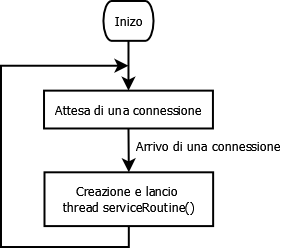
\includegraphics[width=0.5\linewidth]{pictures/runricip.png}
	\caption{Diagramma di flusso per l'esecuzione del metodo Run}\label{fig:riciprun}
\end{figure}
In \fname{fig:riciprun} vediamo come avviene l'esecuzione del metodo \texttt{Run()}. Vediamo come la sua logica sia veramente semplice infatti si tratta di un server socket che attende la ricezione di una connessione. All'arrivo di una nuova connessione esso crea una nuova istanza di thread e tramite questo esegue il metodo \texttt{serviceRoutine()}. Dopo di che si rimette in attesa di una nuova connessione.
\begin{figure}
	\centering
	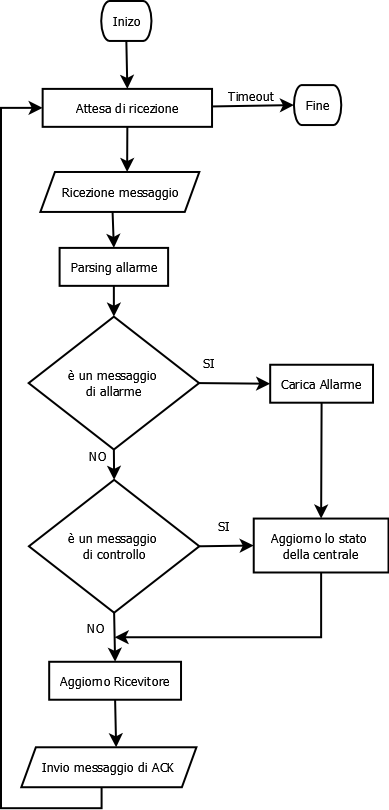
\includegraphics[width=0.5\linewidth]{pictures/servicericip.png}
	\caption{Diagramma di flusso per l'esecuzione del metodo serviceRoutine}\label{fig:servicericip}
\end{figure}
Per quanto riguarda la \texttt{serviceRuntine} il suo funzionamento è illustrato in \fname{fig:servicericip} in questo caso il metodo inizia la sua esecuzione ponendosi in attesa di ricevere un pacchetto, nel caso in cui, dopo un tempo prestabilito, non si riceva alcun pacchetto il metodo va in timeout e termina la sua esecuzione.
Nel caso in cui, invece, si riceva un messaggio si suddivide il messaggio in parti e controllando ognuna delle parti si decide se esso è un messaggio di allarme, allora si invoca il metodo \texttt{CaricaAllarme} se, invece, esso è un messaggio di controllo allora si aggiorna solamente lo stato della centrale per far si che non venga segnalata una anomali di connessione. Fatto ciò si invoca il metodo \texttt{AggiornaRicevitore} che va a modificare il campo di controllo e si invia il messaggio di ACK alla centrale che sta comunicando.
\subsubsection{Ric\_Urmet}\label{algourmet}
Per quanto riguarda il funzionamento del ricevitore AteArgo la logica è leggermente diversa, anche in questo caso analizzeremo in particolare il metodo \texttt{Run()} tramite l'utilizzo dei diagrammi di flusso. In \fname{fig:urmetrun} vediamo il diagramma di flusso che mostra il funzionamento del metodo.
\begin{figure}
	\centering
	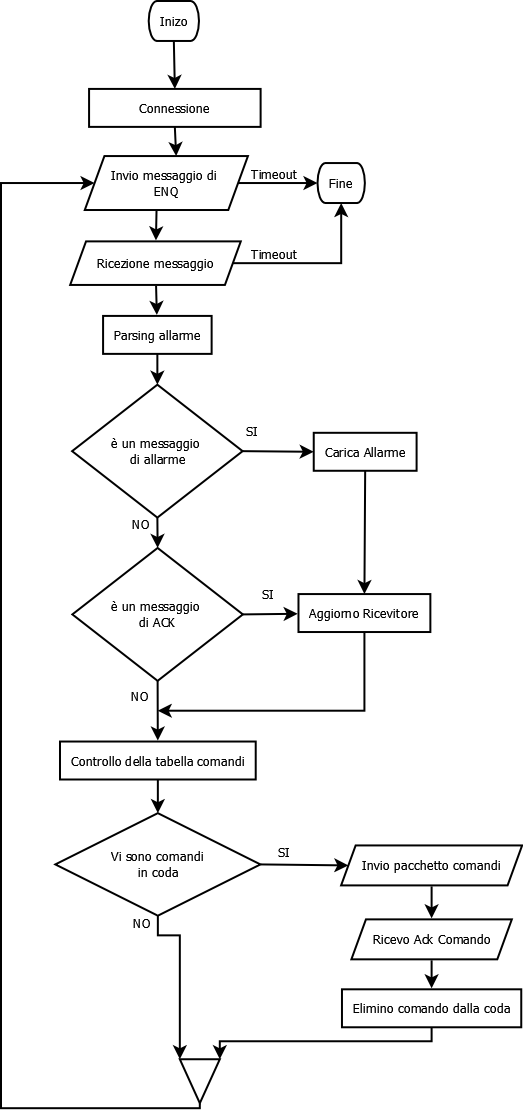
\includegraphics[width=0.7\linewidth]{pictures/runurmet.png}
	\caption{Diagramma di flusso per l'esecuzione del metodo Run della classe Ric\_Urmet}\label{fig:urmetrun}
\end{figure}
Vediamo come la prima operazione che svolge il metodo è quella di connettersi al ricevitore AteArgo, a questo punto il metodo invia un pacchetto di ENQ ed attende la risposta. Quando riceve tale risposta controlla se si tratta di un allarme ed in caso affermativo lo memorizza tramite il \texttt{CaricaAllarme}, nel caso invece sia un pacchetto di ACK aggiorna solamente il ricevitore. Oltre a questo meccanismo che viene ripetuto all'infinito a meno di non avere problemi di connessione, il metodo si occupa anche della gestione dei comandi da inviare alle diverse periferiche, questa caratteristica sarà però analizzata in particolare nel capitolo successivo.
\subsubsection{Ric\_Bentel}
La classe Ric\_Bentel è simile a quella Ric\_IP anche in questo caso il metodo \texttt{Run()} si mette in attesa di una connessione ed il suo comportamento è esattamente uguale a quello della classe Ric\_IP. Quello che cambia è il comportamento del metodo \texttt{serviceRoutine} come viene mostrato in \fname{fig:servicebentel}.
\begin{figure}
	\centering
	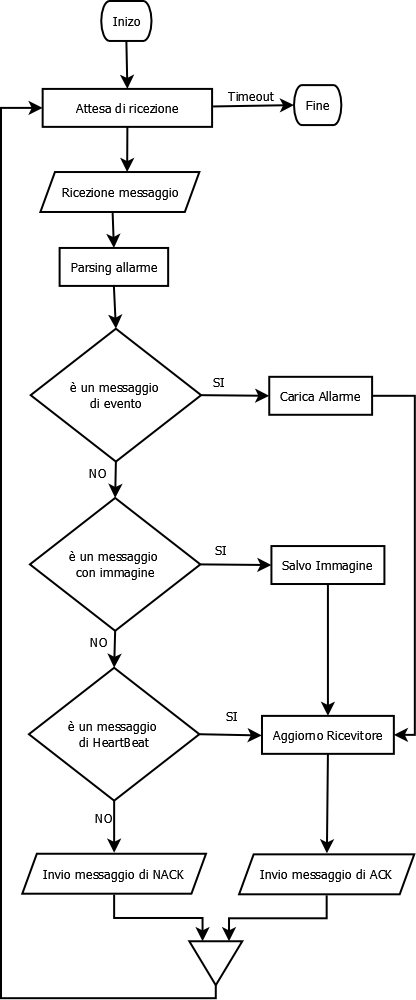
\includegraphics[width=0.7\linewidth]{pictures/servicebentel.png}
	\caption{Diagramma di flusso per l'esecuzione del metodo serviceRoutine della classe Ric\_Bentel}\label{fig:servicebentel}
\end{figure}
In questo caso il metodo si mette in attesa di ricevere un messaggio a questo punto controlla che esso sia uno dei tre possibili messaggi che possono arrivare, nel caso sia un messaggio di evento allora il metodo invoca il \texttt{CaricaAllarme}, nel caso in cui il messaggio contenga un frame di un immagine allora il metodo lo elabora e salva l'immagine, nel caso in cui invece il messaggio sia un semplice HeartBeat allora il metodo invoca \texttt{AggiornaRicevitore} e risponde al messaggio con un ACK dipendente dalla tipologia di messaggio ricevuto e poi si rimette in attesa di ricevere il pacchetto successivo.